\chapter{کاربرد پیچیدگی ارتباطی در پردازش موازی }\label{chapter3}

در این بخش به بررسی محل تقاطع دو علم پردازش موازی و پیچیدگی ارتباطی می‌پردازیم. برای آن که متوجه باشیم چرا پژوهشگران فعال در حوزه پردازش موازی به پیچیدگی ارتباطی اهمیت می‌دهند، لازم است مقداری در مورد پردازش موازی اطلاعات کسب کنیم. در دنیای پردازش موازی، محاسبات داخلی رایگان و محاسبات بین افراد گران است. سه پیچیدگی اصلی در دنیای پردازش موازی شامل تعداد پیغام‌های رد و بدل شده (پیچیدگی پیامی \footnote{Message Complexity})، تعداد بیت‌های ردوبدل شده (پیچیدگی بیتی \footnote{Bit Complexity}) و تعداد دورهای مخابره برای یک مساله و تعدادی کاربر در یک محیط همگام (پیچیدگی دوری\footnote{Round Complexity}) می‌باشد. نکته قابل توجه برای این دو دانش از جایی برمی‌آید که پیچیدگی ارتباطی از دل پردازش موازی استخراج شده‌است و همچنین در بسیاری از مسائل با هم دیگر برابر هستند. لازم است در ادامه انواع مدل‌های پیچیدگی ارتباطی $k$-نفره را بررسی کنیم. 
\section{مدلهای پیچیدگی ارتباطی $k$نفره}

\subsection{مدل تخته‌سیاه}

در این مدل، بازیکنان با یکدیگر از طریق یک تخته سیاه ارتباط برقرار می‌کنند. هر بازیکن در نوبت خودش حق نوشتن روی تخته سیاه را دارد و پروتکل تصمیم می‌گیرد که نوبت چه کسی است. همه بازیکنان می‌توانند تخته را مشاهده کنند. در این مدل و در هنگام شبیه‌سازی، هر بیتی که نوشته می‌شود به $k-1$ بازیکن دیگر مخابره می‌شود. 

\subsection{مدل نفر-به-نفر}
یک گراف ارتباطی\footnote{Communication Graph} مشخص می‌کند که هر بازیکن به چه کسی متصل است و بدون واسطه می‌تواند پیام مخابره کند. برای راحتی کار، گراف‌های ارتباطی را گراف‌های کامل در نظر می‌گیرند که در آن هر دو بازیکن با هم ارتباط دارند. 
\begin{itemize}
	\item [همگام:] در این مدل، مخابرات در دورهای مجزا انجام می‌شو‌د. در هر دور، هر بازیکن یک پیغام می‌فرستد و پیغام‌های ورودی را دریافت می‌کند. 
	\item [ناهمگام:] در این مدل، هیچ دور مخابره‌ای وجود ندارد و هر پیغام در مواقع نیاز فرستاده می‌شود. در این مدل هر بازیکن یک صف دارد که پیغام‌ها‌ی ورودی در آن قرار می‌گیرد.
\end{itemize}
\begin{figure}[h]
	\caption{مثالی از یک مدل نفر-به-نفر 4تایی}
	\centering
	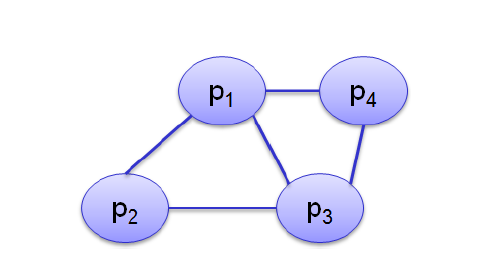
\includegraphics[width=10cm]{3_1.png}
\end{figure}
\subsection{مدل هماهنگ‌کننده}
 در این مدل، که یک حالت خاص از مدل نفر-به-نفر است، تمامی $k$ بازیکن به یک نفر و فقط یک نفر دیگر متصل هستند (در مجموع $k+1$ بازیکن) و بازیکنان از طریق این یک هماهنگ‌کننده با هم در ارتباط هستند. 
 \begin{itemize}
 	\item [همگام:] در هر دور، هر بازیکن یک پیغام به هماهنگ‌کننده می‌فرستد و هماهنگ‌کننده به آنها پاسخ می‌دهد. 
 	\item [ناهمگام:] ارتباط دو نفره بین هرکس از طریق هماهنگ‌کننده و در هر زمان انجام می‌شود. 
 \end{itemize}
\begin{figure}[h]
	\caption{مثالی از یک مدل هماهنگ‌کننده $k$-تایی}
	\centering
	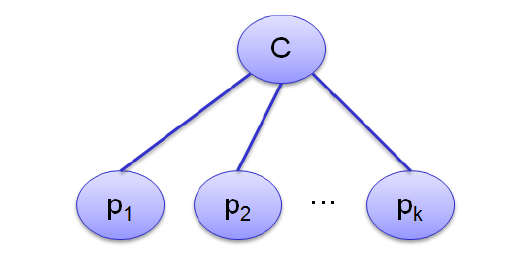
\includegraphics[width=10cm]{3_2.png}
\end{figure}
\section{قرینه‌سازی}
قرینه‌سازی\footnote{Symmetrization} یک تکنیک برای یافتن کمینه در بازی‌های $k$-نفره است.\cite{zhang11} به طور خلاصه، این روش شامل کاهش پروتکل $f_{k}(x_{1},x_{2},...,x_{k})$ به پروتکل   $f_{2}(x,y)$ است. هدف از این تکنیک این است که نشان دهیم محاسبه $f_{k}$ حداکثر به اندازه $k$ برابر $f_{2}$ است. در این مدل، توجه ما روی یک مدل هماهنگ‌کننده با وضعیت تصادفی سکه عمومی\footnote{Public Coin Randomization} است. 

\subsection{تکنیک}
با توجه به یک پروتکل $P_{k}$ که تابع  $f_{k}$ را محاسبه می‌کند، یک پروتکل $P_{2}$ که تابع $f_{2}$ را محاسبه می‌کند می‌سازیم. در مرحله اول باید یک توزیع سخت\footnote{Hard Distribution} از ورودی‌های $f_{2}$ داشته باشیم. آلیس و باب، با استفاده از این توزیع، $k$ ورودی $I_{1}, I_{2}, ..., I_{k}$ را بسازد. به هر $k$ ورودی که از آن توزیع سخت استخراج شده است، قرینه گفته می‌شود اگر هر دوتای آنها را بتوان با هم جابه جا کرد بدون آن که توزیع را عوض کنیم. در این مرحله، آلیس و باب با استفاده از این $k$ ورودی، پروتکل $P_{k}$ را محاسبه می‌کنند. 

\textbf{شبیه‌سازی.} 
آلیس یکی از بازیکنان را به صورت رندوم انتخاب می‌کند. چون وضعیت تصادفی عمومی است، باب می‌د‌‌اند که آلیس کدام بازیکن را انتخاب کرده‌است پس او بقیه بازیکنان را برمی‌د‌ارد و سپس هر دو رفتار بازیکنان را شبیه‌سازی می‌کنند. فرض کنید که آلیس بازیکن $P_{i}$ را انتخاب کرده‌است. در در نتیجه هر پیغامی که بین بازیکن $i$م و بقیه بازیکنان رد و بدل می‌شود، بین آلیس و باب هم رد و بدل می‌شود. بقیه پیغام‌ها در این مدل به عنوان پیچیدگی ارتباطی حساب نمی‌شوند. 
 
 
\textbf{کمینه.}
 هزینه پروتکل $P_{2}$ را  $Cost(P_{2})$ و هزینه پروتکل $P_{k}$ را $Cost(P_{k})$ بنامید. از آنجایی که ورود‌ی‌ها قرینه هستند، از نظر امید ریاضی، $P_{2}$ حداکثر $1/k$ کل بیت‌هایی را مخابره می‌کند که $P_{k}$ می‌کرده است. این بدین علت است که به صورت یکنواخت، امکان انتخاب هر بازیکن دیگر برای آلیس وجود داشت، در نتیجه امید ریاضی یالی که آلیس در مدل گرافی معادل انتخاب کرده‌است، $1/k$ کل یال‌ها اطلاعات رد و بدل می‌کرده است. در نتیجه
\begin{equation}
	{E}[Cost(P_{2})] \leq (1/k) {E}[Cost(P_{k})]
\end{equation}
\begin{figure}[h]
	\caption{شبیه‌سازی مدل -$k$تایی}
	\centering
	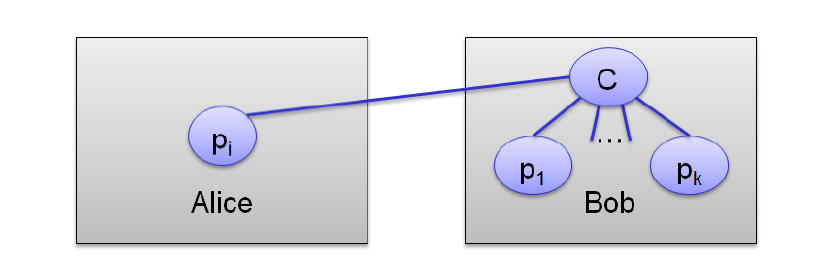
\includegraphics[width=10cm]{3_3.png}
\end{figure}
\subsection{پیشنیازها} %TODO Better title
همانطور که در \autoref{dist_rand} بیان شد، پیچیدگی ارتباطی توزیعی \footnote{Distributional communication complexity} $D_{\epsilon}^{\mu}$ با خطای $\epsilon$ و توزیع ورودی $\mu$ به صورت زیر تعریف می‌شود:
\begin{equation}
	D_{\epsilon}^{\mu} = \min_{P} \max_{x} Cost(P(x))\mu (x)
\end{equation}
در حالی که $Cost(P(x))$ هزینه پروتکل $P$ بر روی ورودی $x$ است. به عبارتی دیگر، $D_{\epsilon}^{\mu}$ بدترین حالت مخابره برای یک ورودی (بدترین ورودی) برای بهترین پروتکل است. 

از آنجایی که مخابره $k$-نفره $k$ برابر امید مخابره 2 نفره است، مفهومی از امید باید در پیچیدگی ارتباطی تعریف شود. امید پیچیدگی ارتباطی توزیعی ${E}[D_{\epsilon}^{\mu}]$ با خطای $\epsilon$ و توزیع $\mu$ به صورت زیر است
\begin{equation}
 {E}[D_{\epsilon}^{\mu}] = \min_{P} {E}_{x}[Cost(P(x))\mu(x)].
\end{equation}
در نتیجه این تعریف و قضیه مین‌ومکس یائو\footnote{Yao's Minmax Theorem} می‌توان گفت:
\begin{equation}
	R_{\epsilon} \geq D^{\mu}_{\epsilon} \geq {E}[D_{\epsilon}^{\mu}]
\end{equation}
حال با اتکا به قضیه نظریه اطلاعاتی زیر، تعدادی مثال مطرح می‌کنیم.\cite{zhang11}

 
{قضیه:}
 فرض کنید آلیس و باب هر کدام یک ورودی یکنواخت $n$ بیتی دارند. برای آن‌که آلیس با احتمال $(1-\epsilon)$ ورودی باب را بداند، لازم است امیداً باب $(1-\epsilon)n$ بیت بفرستد.

\section{مثال}
\subsection{$k-XOR$: هماهنگ‌کننده}
مساله $k-XOR$ در مدل هماهنگ‌کننده به صورت زیر است:
\begin{enumerate}
	\item بازیکن‌ها $p_{1},p_{2},p_{3},...,p_{k}$ هستند. 
	\item ورودی‌ها رشته‌های $n$ بیتی به صورت $I_{1},I_{2},I_{3},...,I_{k}$ هستند.
	\item خروجی یک رشته $n$ بیتی است که بیت $i$م، $XOR$ بیت $i$م ورودی‌هاست.
\end{enumerate}
هدف استفاده از پروتکل $P_{k}$ برای طراحی پروتکل $P_{2}$ است. بعد از آن، از کمینه پروتکل $2-XOR$ استفاده می‌کنیم تا یک کمینه روی مخابره $k$-نفره بیابیم. 

\textbf{ساخت ورودی‌های قرینه برای $P_{k}$:} 
اول از همه باید یک توزیع سخت برای ورودی مخابره دونفره پیدا کنیم که به اندازه کافی برای یافت کمینه این مخابره سخت باشد. برای این کار توزیع یکنواخت به اندازه کافی سخت است. در نتیجه، آلیس به صورت یکنواخت تصادفی  بازیکن $p_{i}$ را انتخاب می‌کند و $I_{i}$ را برابر با ورودی خودش یعنی $x$ قرار می‌دهد. باب نیز به صورت تصادفی $k-1$ رشته $n$ بیتی را به صورتی می‌سازد که 
\begin{equation}
	\{I_{j} \, | \, j \ne i \} \quad s.t. \, \, XOR(I_{1},I_{2},...,I_{i-1},I_{i+1},...,I_{k}) = y
\end{equation}
که در آن $y$ ورودی باب است. ورودی‌ها به وضوح قرینه هستند. آلیس بازیکن $i$م و باب همه $k-1$ بازیکن دیگر و همینطور هماهنگ‌کننده را شبیه‌سازی می‌کند.

\textbf{کمینه:}
از آنجایی که ورودی‌ها قرینه هستند، امید مقدار مخابره بین $p_{i}$ و هماهنگ‌کننده $1/k$ برابر کل مخابره پروتکل $P_{k}$ است. در نتیحه، $Cost(P_{2}) \leq (1/k)E[Cost(P_{k})]$ است و یا $Cost(P_{k}) \geq kE[Cost(P_{2)}]$. حال لازم است یک کمینه برای $kE[Cost(P_{2)}]$ بیابیم. 

با داشتن $XOR(x,y)$، آلیس می‌تواند ورودی باب یعنی $y$ را بازیابی کند. طبق قضیه نظریه اطلاعاتی، باب باید امیداً $n$ بیت بفرستد که یعنی $kE[Cost(P_{2})] \geq n$ و در نتیجه، $Cost(P_{k}) \geq nk$.    
\subsection{$k-XOR$: تخته‌سیاه}
مساله مثال قبل را در نظر بگیرید. مدل ارتباطی را به مدل تخته‌سیاه عوض کنید. ساخت ورودی‌ها و شبیه‌سازی با تغییر مدل نیز تغییر می‌یابند. 

\textbf{آماده‌سازی شبیه‌سازی:} 
آلیس و باب هرکدام به صورت یکنواخت تصادفی بازیکن $p_{i}$ و $p_{j}$ را انتخاب می‌کنند ($i \ne j $). آلیس همه‌ بازیکن‌ها به جز بازیکن $j$ را شبیه‌سازی می‌کند. همینطور باب، همه بازیکن‌ها به جز بازیکن $i$ را شبیه‌سازی می‌کند. در نتیجه، هر بازیکنی به جز $i$ و $j$ توسط هر دو طرف شبیه‌سازی می‌شود. 
\begin{figure}[h]
	\caption{شبیه‌سازی دوتایی آلیس و باب برای پروتکل $k$تایی $k-XOR$ در مدل تخته‌سیاه}
	\centering
	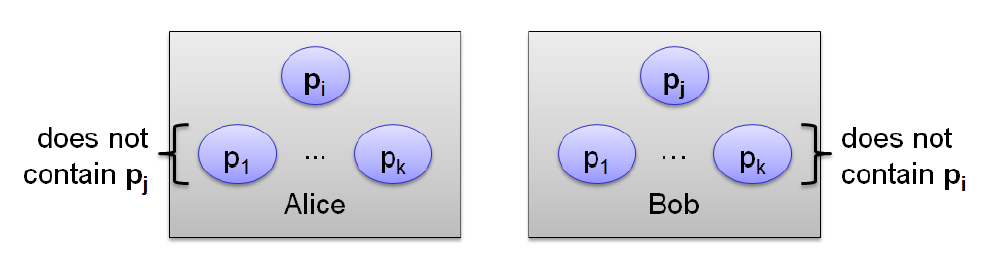
\includegraphics[width=10cm]{3_4.png}
\end{figure}

\textbf{ساخت ورودی قرینه}
مانند حالت قبل، توزیع یکنواخت یک توزیع سخت محسوب می‌شود. آلیس مقدار $I_{i}$ را برابر با $x$ قرار می‌دهد. باب نیز مقدار $I_{j}$ را برابر با $y$ قرار می‌دهد. بقیه ورودی‌ها به صورت تصادفی با استفاده از سکه عمومی مشترک مقداردهی می‌شوند. مشخص است که ورودی‌های ساخته شده قرینه هستند. 

\textbf{اجرای شبیه‌سازی:}
هربار بازیکن $i$م بیتی را روی تخته می‌نویسد، بقیه افراد باید مقدار نوشته شده را بتوانند بخوانند. اما از آنجایی که باب $p_{i}$ را شبیه سازی نمی‌کند، تا زمانی که آلیس همان‌چیزی که $p_{i}$ می‌نویسد را روی تخته‌‌سیاه ننویسید، یک بازیکن مانند $p_{j}$ از مخابرات $p_{i}$ آگاه نمی‌شود. پس هرگاه در پروتکل $P_{k}$، $p_{i}$ اطلاعاتی را مخابره کند، آلیس نیز باید آن‌ را مخابره کند. این مساله برای باب و بازیکن $p_{j}$ نیز صادق است. ولی مخابرات بقیه بازیکنان نیازی به نوشته شدن روی تخته‌سیاه ندارد چرا که هر دو طرف آن‌ها را شبیه‌سازی می‌کنند. 

 \textbf{پیچیدگی ارتباطی:} 
 از آنجایی که ورودی‌ها قرینه هستند و آلیس و باب تنها زمانی مخابره می‌کنند که دوتا از بازیکنان مخابره می‌کنند، امید مقدار مخابره برای $P_{2}$ حداکثر $\frac{k}{2}$ برابر مخابره برای $P_{k}$ است. در نتیجه، $E[Cost(P_{2})] \leq (2\k)Cost(P_{k})$ است که برابر است با $Cost(P_{k}) \geq (k/2)E[Cost(P_{2})]$. طبق قضیه نظریه اطلاعات، $E[Cost(P_{2})] = n$. در نهایت، $Cost(P_{k}) \geq \frac{nk}{2}$.
\subsection{$k-DISJ$ بدون قرینه‌سازی}
مساله اشتراک\footnote{Disjointness} به صورت گسترده در مخابرات دوتایی استفاده شده‌است و بسیاری از مسائل به این مساله کاهش یافته‌اند. این درحالی است که نسخه $k$-تایی این مساله، یعنی مساله‌ای که $k$ بازیکن خروجی 1 می‌دهند اگر و تنها اگر همه بازیکنان در یک عضو اشتراک داشته باشند، این خاصیت را ندارد. برای این که این مساله را نشان دهیم، یک پروتکل با پیچیدگی $O(nk)$ طراحی می‌کنیم. درنهایت مساله‌ای را معرفی می‌کنیم که کمینه بیشتری دارد. \cite{arkadev14} 

در مرحله اول، همه بازیکنان درخت پوشای کمینه گراف ارتباطی را به صورت محلی محاسبه می‌کنند. یک بازیکن دلخواه مانند $p_{root}$ را به عنوان ریشه درخت در نظر بگیرید. هر بازیکنی که برگ است، ورودی خود را به پدر خود می‌فرستد. پدر، اشتراک مجموعه خود و فرزندانش را محاسبه می‌کند و برای پدر خود می‌فرستد. این درخت پوشای کمینه دقیقا $k-1$ یال دارد که هر کدام $n$ بیت داده جابه‌جا می‌کنند. در پایان پروتکل، $p_{root}$ اشتراک همه را می‌داند و می‌تواند خروجی را به همه اطلاع دهد. پیچیدگی ارتباطی این پروتکل، $(k-1)(n+1)$ است.  

حال مساله‌ای مانند $k-DIST$، که در آن بازیکنان خروجی $1$ می‌دهند اگر و تنها اگر هردوتایی از ورودی‌ها متمایز باشد، در نظر بگیرید. می‌توان نشان داد که پروتکل بهینه برای این مساله وقتی است که همه بازیکنان ورودی‌شان را برای یک دیگر می‌فرستند. در یک گراف ارتباطی با قطر $d$، یعنی بلندترین کوتاه‌ترین مسیر، تعداد مخابره مورد نیاز برای آگاه شدن همه از ورودی یک‌دیگر برابر با $O(nkd)$ است. اگر گراف کامل باشد، $d$ برابر با $1$ است و بزگترین مقدار می‌تواند $k$ باشد که کمینه $O(nk^{2})$ را می‌دهد. 

 از دیگر مسائل سخت می‌توان به مسائلی اشاره کرد که در یک مخابره $k$تایی، هر بازیکن یک زیرگراف مانند $H_{k}$ از یک گراف مانند $G$ را داشته باشند و بخواهند تصمیم بگیرند که درجه یک راس مشخص در $G$ چند است، آیا $G$ دور دارد یا خیر، مثلث دارد یا خیر، متصل است یا خیر و آیا دوبخشی است یا خیر. \cite{arkadev14}
 